\chapter{qiita2reviewの使い方}
\label{chap:howtoQiita2Review}

Re:VIEW を apache で動かす
http://qiita.com/nanbuwks/items/dd15819ec7798a9eca7b

で書いた、qiita から pdfを作るシステム。
これを使う前提でのQiitaの記事の書き方。

\begin{reviewimage}
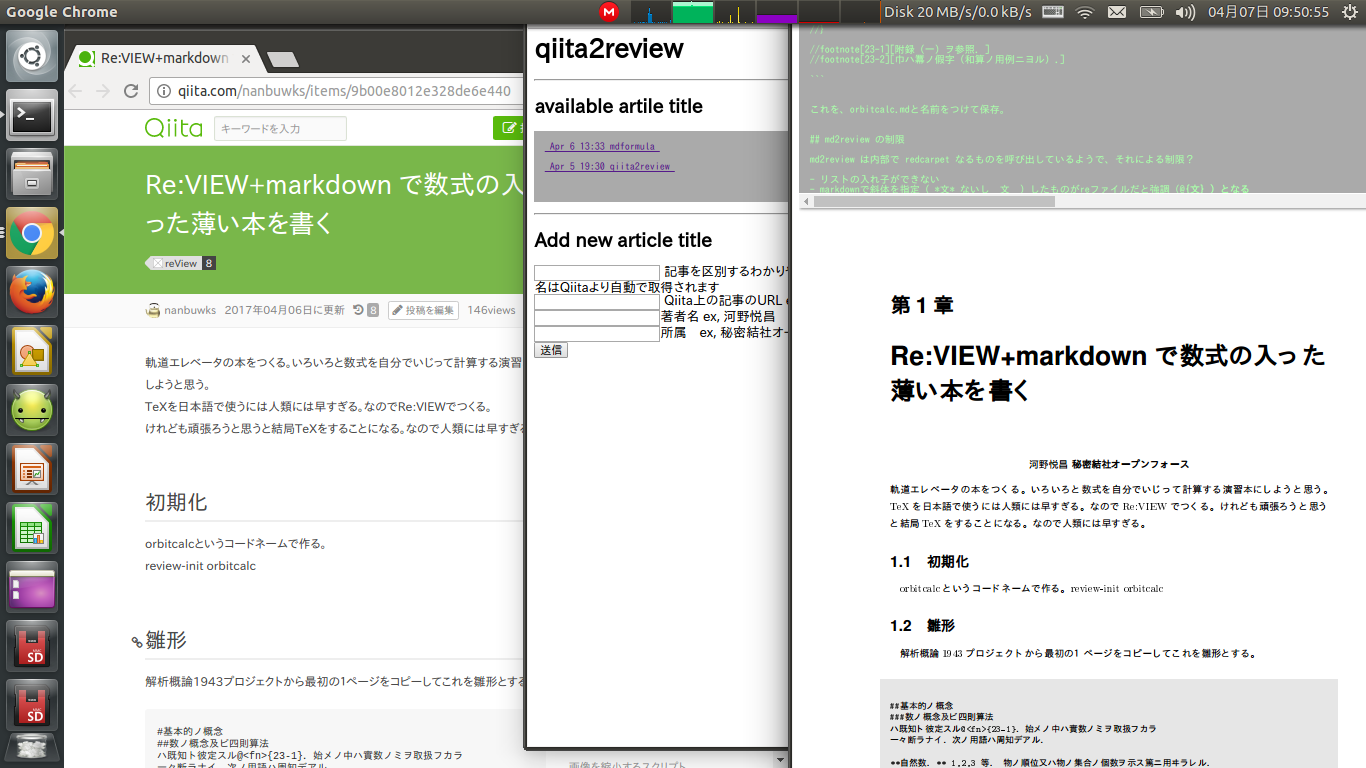
\includegraphics[width=\maxwidth]{./images/80cbc196-d4ef-b880-733c-54d0a8aa45bb.png}
\caption{Screenshot from 2017{-}04{-}07 09{-}50{-}56.png}
\label{image:howtoQiita2Review:80cbc196-d4ef-b880-733c-54d0a8aa45bb}
\end{reviewimage}

\section{qiita2review とは}
\label{sec:1-1}

\begin{itemize}
\item Qiita で記事を執筆してもらってRe:VIEWでPDFにするオンラインシステム。
\item グループ作業で技術情報をマルチ展開するために。
\item Qiita だと学習コスト少、画像楽だし数式も使える。
\item PDF作ると同時にちゃんとしたWebコンテンツを公開できる。
\end{itemize}

\section{管理者がはじめにやること}
\label{sec:1-2}

サーバにインストール、認証設定、サーバアドレスの執筆者への周知。

\section{執筆者がやること}
\label{sec:1-3}

\subsection*{Qiitaに記事を書く}
\addcontentsline{toc}{subsection}{Qiitaに記事を書く}
\label{sec:1-3-1}

後々PDFにするために、ちょっと気をつける点。

\subsubsection*{画像}
\label{sec:1-3-1-1}

画像はそのままだと100\%になり、紙媒体では大きすぎることが多い。縮小設定をしておく。
通常の画像は

\begin{reviewemlist}
![ファイル名](images/......8d78.jpeg)
\end{reviewemlist}

のようになってますが

\begin{reviewemlist}
[]( scale=0.5 )![ファイル名](https://qiita{-}image{-}store.s3.amazonaws.com/0/......8d78.jpeg)

\end{reviewemlist}

のように頭に\texttt{scale=0.5 )}をつけると、Qiitaでは100\%,PDFにしたときには50\%サイズになります。

\subsubsection*{Re:VIEWの制限}
\label{sec:1-3-1-2}

PDF化に使用しているRe:VIEW受け付けない書式にならないように注意
{-} コメントの入れ子
{-} コードブロック開始前に改行を入れる

コードブロック開始前に改行がない場合、Markdownとしてもヘンになることが多いので改行を入れる習慣をつけよう。

\subsection*{Qiitaに記事が書けたら}
\addcontentsline{toc}{subsection}{Qiitaに記事が書けたら}
\label{sec:1-3-2}

PDF化の確認をします。

qiita2reviewサーバページから、記事一覧が見えます。

画面下部の
「Add new article title」
のフォームに入力して送信すると新しい記事が登録できる。

(認証が必要)

Qiitaの1記事ごとにPDFになる。別刷りのようなイメージ。

\section{原稿が集まったら}
\label{sec:1-4}

本としての装丁は管理者が行います。
1記事になっているものはそれぞれ章にして、まとめて1冊としてレンダリング→印刷
管理者のお仕事となります。今のところはサーバにsshログインしてRe:VIEWを使って手作業です。
